\section{Kanban - ein Beispiel}

\subsection*{Kanban - ein Beispiel}

\begin{frame}
	\frametitle{Inhalt des Vortrags?}
		\begin{figure}[ht]
			
\includegraphics[width=6.5cm]{Bilder/fragerunde.png}
		\end{figure}
\end{frame}

\begin{frame}
	\frametitle{Unser Ziel}
	\begin{exampleblock}{Ziel}
		Unterschiede der Verfahren \emph{Push} und \emph{Pull} erleben, Metriken anwenden und vergleichen.
	\end{exampleblock}
\end{frame}

\begin{frame}
	\frametitle{Unsere Produktion}
	\begin{exampleblock}{Papierflieger bauen}
		Lean Production: Papierflieger bauen im Push- und Pull-Verfahren.
	\end{exampleblock}
	\begin{itemize}[<+->]
		\item 1 Manager/Projektleiter
		\item 1 Logistiker
		\item 4 Projektmitarbeiter
		\item (x) Beobachter
	\end{itemize}
\end{frame}
\begin{frame}
	\frametitle{Gruppen}
	\begin{exampleblock}{Eure Aufgabe}
		Gruppe bilden 6 + Beobachter
	\end{exampleblock}
	\pause
	\begin{itemize}[<+->]
			\item Rollen verteilen
			\item Projektmitarbeiter auf eine Seite (immer 1 Platz frei)
			\item Alle anderen stellen sich auf die andere Seite
		\end{itemize}
\end{frame}
\begin{frame}
	\frametitle{Eure Aufgabe Push-Vorgehen}
	\begin{exampleblock}{Aufgabe}
		Das folgende Szenario wird \textbf{5 Minuten} durchgespielt.
	\end{exampleblock}
	\begin{itemize}[<+->]
		\item Vier Prozessschritte für 4 Projektmitarbeiter
		\item Jeder Prozessschritt hat Ein- und Ausgang
		\item Prozess\textbf{kette} -> FIFO
		\item Logistiker transportiert Ware zwischen Ein- und Ausgang
		\item Manager/Projektleiter steuert verbal den Logistiker und achten auf Zeiten
		\item Manager/Projektleiter fügt in Minute 0:30 und 3:30 ein farbiges Papier ein um Durchlaufzeit zu messen (Zeit stoppen!)
		\item Beobachter beobachten den Verlauf und notieren Auffälligkeiten
		\item  Manager/Projektleiter und Beobachter füllen Metrikliste aus
	\end{itemize}
\end{frame}
\begin{frame}
	\begin{figure}[ht]
		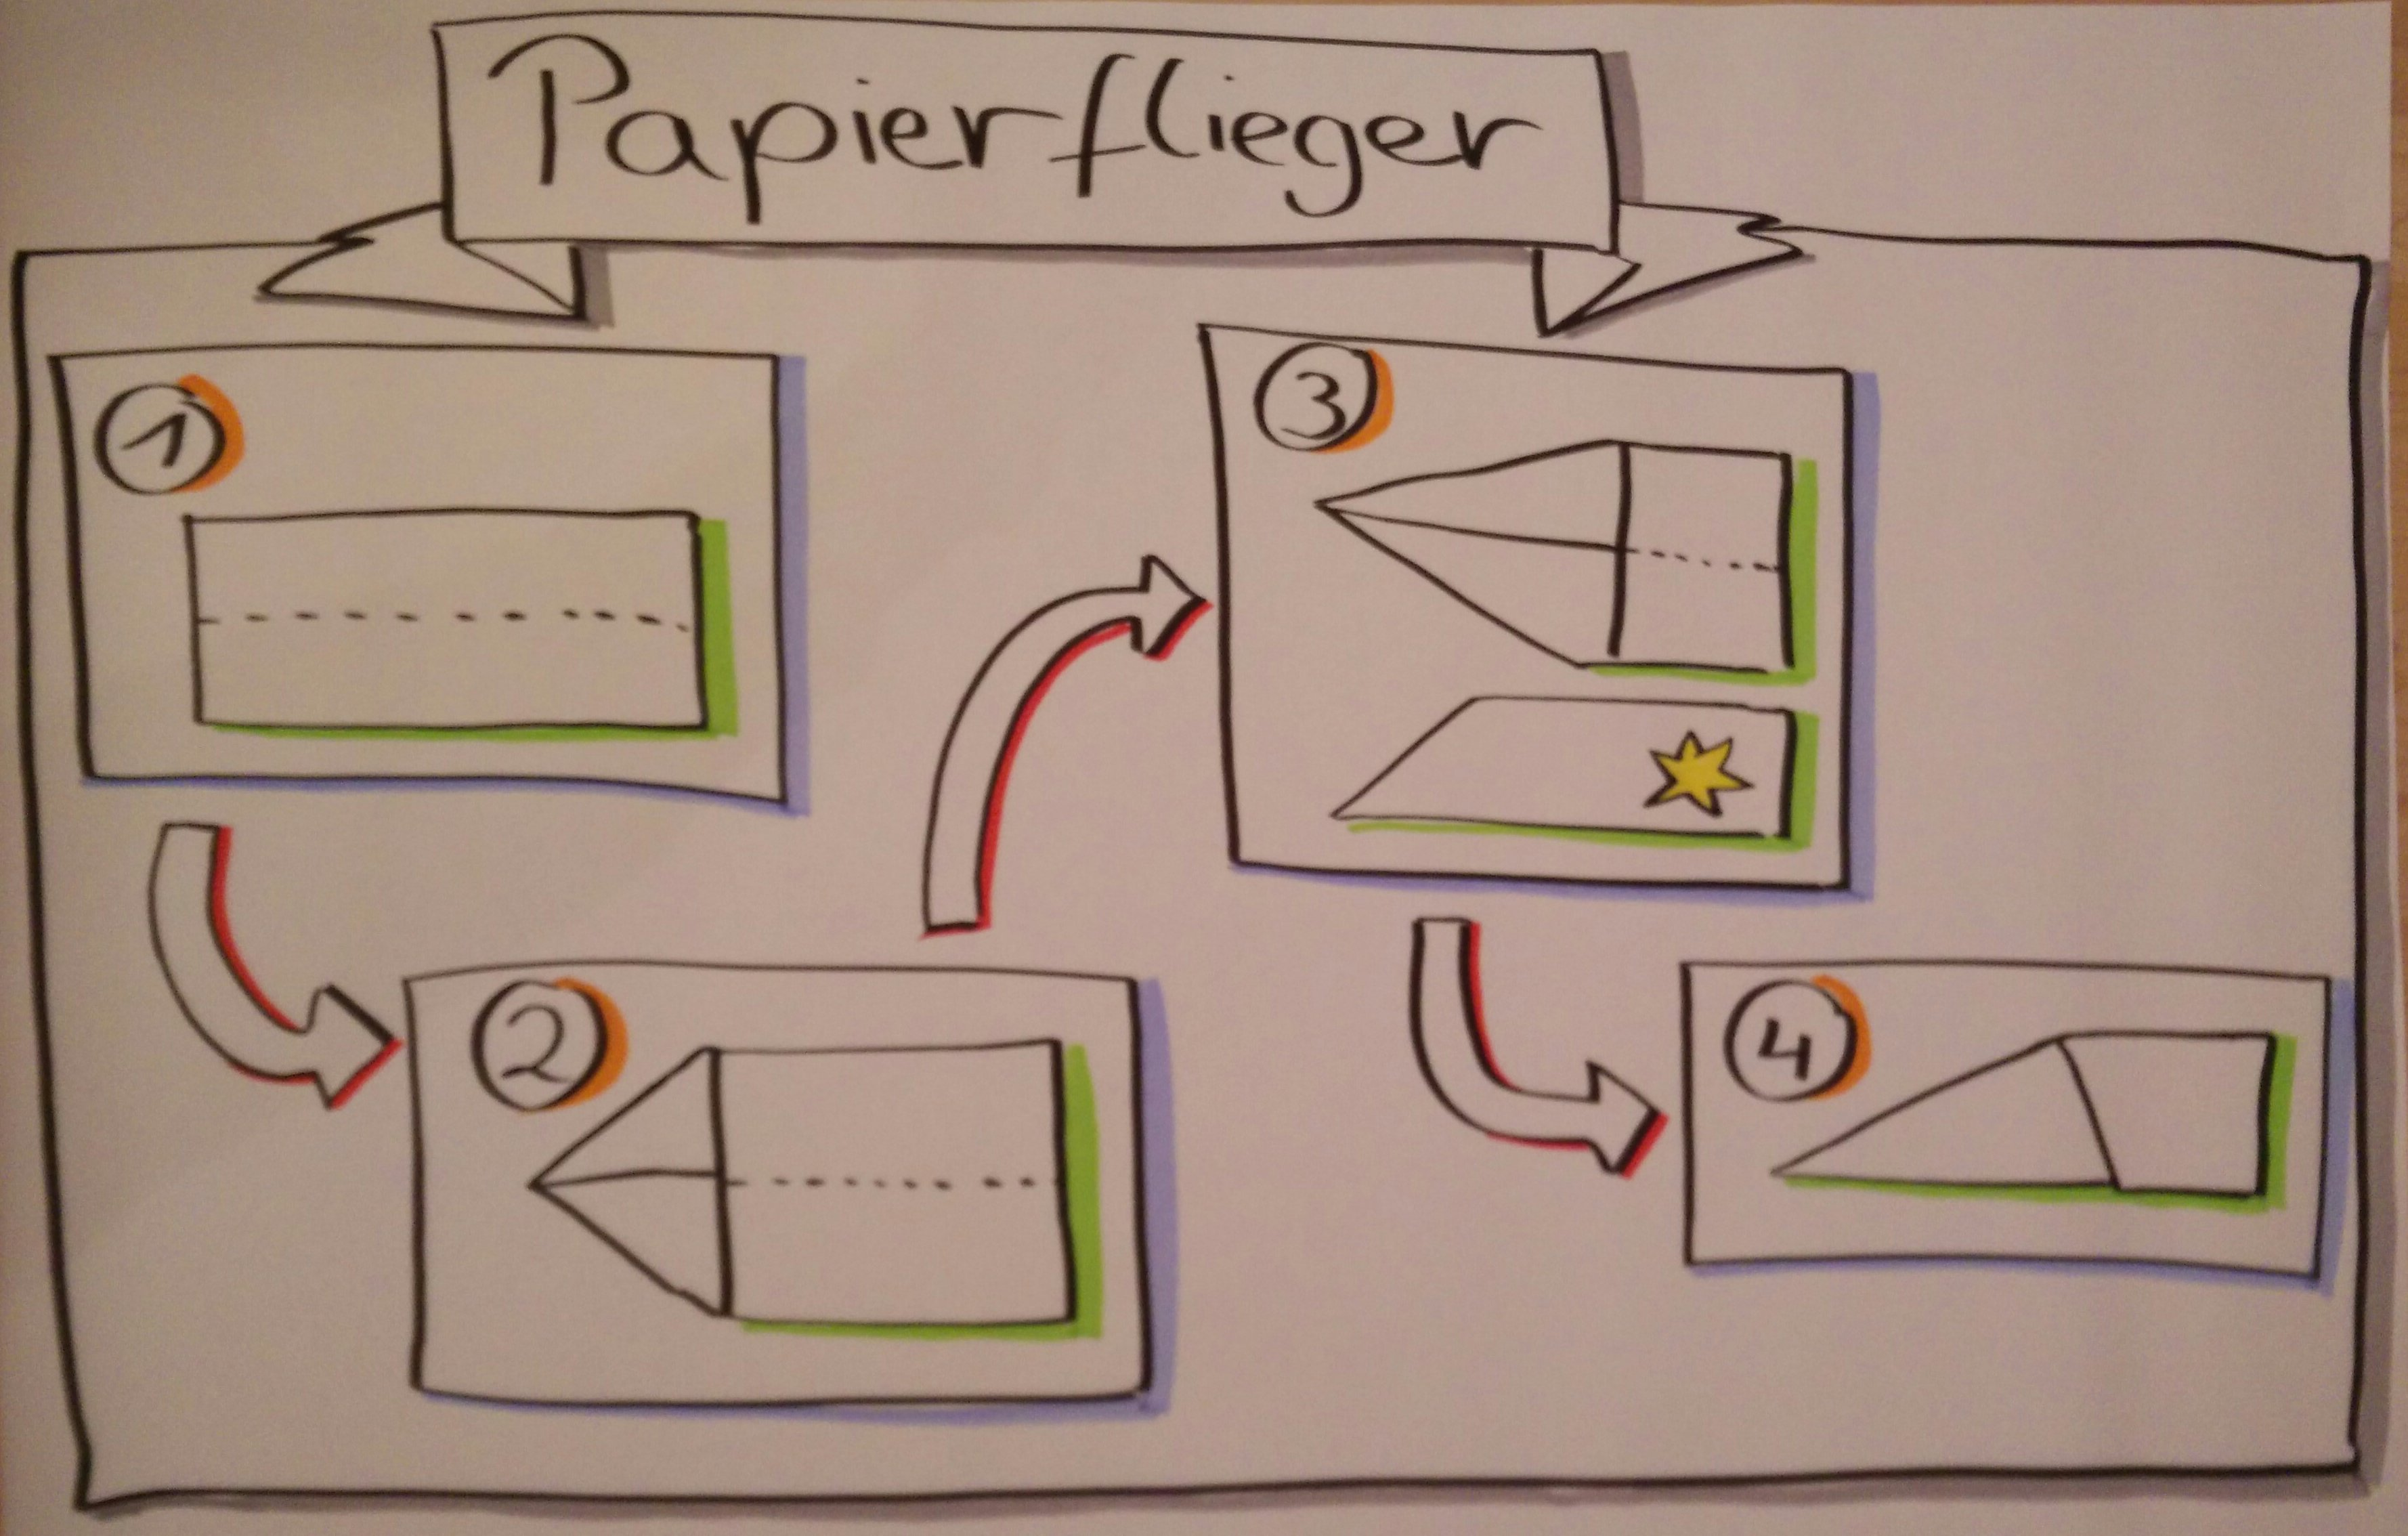
\includegraphics[width=10.9cm]{Bilder/papierflieger.jpg}
	\end{figure}
\end{frame}
\begin{frame}
	\frametitle{Eure Aufgabe Pull-Vorgehen}
	\begin{exampleblock}{Aufgabe}
		Das folgende Szenario wird \textbf{5 Minuten} durchgespielt.
	\end{exampleblock}
	\begin{itemize}[<+->]
		\item Vier Prozessschritte für 4 Projektmitarbeiter
		\item Jeder Prozessschritt hat \textbf{kombinierten} Ein- und Ausgang
		\item Kombinierte Ein- und Ausgänge dienen als Übergabepunkte
		\item Projektmitarbeiter nimmt nur \emph{neues} Material, wenn sein \emph{Ausgang} leer ist
		\item Manager fügt in Minute 0:30 und 3:30 ein farbiges Papier ein um Durchlaufzeit zu messen
		\item  Manager/Projektleiter und Beobachter füllen Metrikliste aus
	\end{itemize}
\end{frame}

\begin{frame}
	\frametitle{Auswertung}
	\begin{exampleblock}{Metriken}
		Auswertung und Besprechung der Ergebnisse einer Gruppe
	\end{exampleblock}
\end{frame}
\begin{frame}
	\frametitle{Fazit Push-Vorgehen}
	\begin{itemize}[<+->]
		\item Viele unfertige Produkte
		\item Lange Durchlaufzeiten
		\item Bei laufender Änderung hoher Ausschuss
		\item Spätes Erkennen von Fehlern teuer
		\item Hoher Aufwand für Logistik und Management
	\end{itemize}
\end{frame}
\begin{frame}
	\frametitle{Fragen und Antworten}
	\begin{figure}[ht]
		
\includegraphics[width=8.0cm]{Bilder/fragenantwort.png}
	\end{figure}
\end{frame}